\chapter{Natural Transformations}
\label{chap:naturals}

\epigraph{
  ... and \emph{functor} has been defined in order to be able to
  define \emph{natural transformation}.
}{---\textcite[18]{maclane-1998}}

In this chapter we explore natural transformations and their relation
to polymorphic functions in Haskell. Despite their name, natural
transformations might be ``a first stumbling block'' in the study of
category theory, ``simply because the examples tend to raise the level
of mathematical sophistication'' \parencites[433]{poigne-1992}. But
natural transformations are indeed natural, especially in functional
programming. It is typical to explain this idea with examples of
parametrically polymorphic functions such as appending an element to a
list, extracting the first component of a pair, reversing a list,
among others.

In Haskell, one such function is the \texthaskell{head} function,
which extracts the first element of a list\footnote{Note that this is
  not the standard Haskell \texthaskell{head} function.}:
\begin{codehaskell}
head :: [a] -> Maybe a
head []    = Nothing
head (x:_) = Just x
\end{codehaskell}
This is not any function, but a function between functors. More
specifically, it is a function from the \texthaskell{[]} (list)
functor into the \texthaskell{Maybe} functor. Besides, it is not just
a function, but rather a family of functions indexed by Haskell types.

The \texthaskell{head} function is natural or uniform in the sense
that, given two types \texthaskell{a} and \texthaskell{b}, a function
\texthaskell{f :: a -> b}, and a list of elements of \texthaskell{a},
mapping the function over the list and then extracting the first
element of the result is the same as extracting the first element of
the list and then mapping the function over the result:
\begin{codehaskell}
head . fmap f = fmap f . head
\end{codehaskell}
That is, the diagram in Figure \ref{fig:naturality-head-haskell} is
commutative.

\begin{figure}[htb]
  \begin{center}
    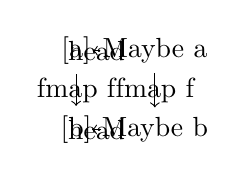
\begin{tikzpicture}
      \node (f a)                {\texthaskell{[a]}};
      \node (f b) [below of=f a] {\texthaskell{[b]}};
      \node (g a) [right of=f a] {\texthaskell{Maybe a}};
      \node (g b) [below of=g a] {\texthaskell{Maybe b}};

      \draw [->] (f a) to node [swap] {\texthaskell{fmap f}} (f b);
      \draw [->] (g a) to node        {\texthaskell{fmap f}} (g b);

      \draw [->] (f a) to node        {\texthaskell{head}}   (g a);
      \draw [->] (f b) to node [swap] {\texthaskell{head}}   (g b);
    \end{tikzpicture}
  \end{center}
  \caption{Naturality of the \texthaskell{head} function.}
  \label{fig:naturality-head-haskell}
\end{figure}

Even if this is an intuitive property of the \texthaskell{head}
function and proving it is quite simple, this property says a lot
about the behavior of all the functions that are part of the family
defined by \texthaskell{head}. Most importantly, all of these facts
are abstracted by natural transformations.

\section{Natural Transformations}
\label{sec:naturals}

Having defined categories and functors (morphisms of categories), let
us now define natural transformations (morphisms of functors).

\begin{definition}
  \label{def:natural}

  %% \parencites[16]{maclane-1998}[435--436]{poigne-1992}

  Let $\func{F}$ and $\func{G}: \cat{C} \to \cat{D}$ be functors for
  two categories $\cat{C}$ and $\cat{D}$. A natural transformation
  \begin{equation*}
    \nat{\tau}: \func{F} \to \func{G}: \cat{C} \to \cat{D}
  \end{equation*}
  assigns to each object $a$ in $\cat{C}$ a morphism $\natO{\tau}{a}:
  \funcO{F}(a) \to \funcO{G}(a)$ in $\cat{D}$, called a component of
  the natural transformation, such that, for all morphisms $f: a \to
  b$ in $\cat{C}$,
  \begin{equation}
    \label{eq:naturality}
    \natO{\tau}{b} \comp \funcM{F}(f) = \funcM{G}(f) \comp \natO{\tau}{a}
    \text{,}
  \end{equation}
  that is, the diagram in Figure \ref{fig:naturality} is commutative.

  \begin{figure}[htb]
    \begin{center}
      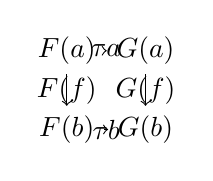
\begin{tikzpicture}
        \node (f a)                {$\funcO{F}(a)$};
        \node (f b) [below of=f a] {$\funcO{F}(b)$};
        \node (g a) [right of=f a] {$\funcO{G}(a)$};
        \node (g b) [below of=g a] {$\funcO{G}(b)$};

        \draw [->] (f a) to node [swap] {$\funcM{F}(f)$}   (f b);
        \draw [->] (g a) to node        {$\funcM{G}(f)$}   (g b);

        \draw [->] (f a) to node        {$\natO{\tau}{a}$} (g a);
        \draw [->] (f b) to node [swap] {$\natO{\tau}{b}$} (g b);
      \end{tikzpicture}
    \end{center}
    \caption{Naturality of a natural transformation.}
    \label{fig:naturality}
  \end{figure}

\end{definition}

As an example, the identity morphisms of a category are the components
of a natural transformation, and, interestingly, the identity axiom of
the category is the naturality of the transformation.

\begin{example}
  \label{ex:natural-identity}

  Given a category $\cat{C}$, the identity natural transformation
  $\id: \func{I} \to \func{I}: \cat{C} \to \cat{C}$ assigns to each
  object $a$ the identity morphism $\idO{a}: a \to a$. This is a
  natural transformation from and into the identity endofunctor (see
  Example \ref{ex:functor-identity}). Naturality is the commutativity
  of the diagram in Figure \ref{fig:natural-identity}, which holds by
  \eqref{eq:category-identity}. More explicitly, naturality
  corresponds to the commutativity of the diagram in Figure
  \ref{fig:natural-identity-explicit}, which includes the identity
  endofunctor.

  \begin{figure}[htb]
    \begin{center}
      \begin{subfigure}[t]{0.45\linewidth}
        \begin{center}
          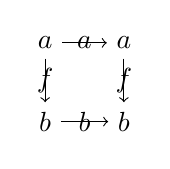
\begin{tikzpicture}
            \node (f a)                {$a$};
            \node (f b) [below of=f a] {$b$};
            \node (g a) [right of=f a] {$a$};
            \node (g b) [below of=g a] {$b$};

            \draw [->] (f a) to node [swap] {$f$}       (f b);
            \draw [->] (g a) to node        {$f$}       (g b);

            \draw [->] (f a) to node        {$\idO{a}$} (g a);
            \draw [->] (f b) to node [swap] {$\idO{b}$} (g b);
          \end{tikzpicture}
        \end{center}
        \caption{}
        \label{fig:natural-identity}
      \end{subfigure}
      \begin{subfigure}[t]{0.45\linewidth}
        \begin{center}
          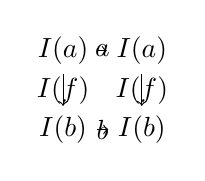
\begin{tikzpicture}
            \node (f a)                {$\funcO{I}(a)$};
            \node (f b) [below of=f a] {$\funcO{I}(b)$};
            \node (g a) [right of=f a] {$\funcO{I}(a)$};
            \node (g b) [below of=g a] {$\funcO{I}(b)$};

            \draw [->] (f a) to node [swap] {$\funcM{I}(f)$} (f b);
            \draw [->] (g a) to node        {$\funcM{I}(f)$} (g b);

            \draw [->] (f a) to node        {$\idO{a}$}      (g a);
            \draw [->] (f b) to node [swap] {$\idO{b}$}      (g b);
          \end{tikzpicture}
        \end{center}
        \caption{}
        \label{fig:natural-identity-explicit}
      \end{subfigure}
    \end{center}
    \caption{Naturality of the identity natural transformation.}
  \end{figure}

\end{example}

As an example of natural transformations as morphisms of functors, the
identity and power set functors are related in a natural manner.

\begin{example}
  \label{ex:natural-identity-power-set}

  %% \parencite[11]{marquis-2013}

  In $\set$, $\nat{\eta}: \func{I} \to \func{P}: \set \to \set$ is a
  natural transformation which assigns to each set $A$ a function
  $\natO{\eta}{A}: \funcO{I}(A) \to \funcO{P}(A)$ such that, for all
  $x \in A$,
  \begin{equation}
    \label{eq:eta}
    \natO{\eta}{A}(x) = \{x\}
    \text{.}
  \end{equation}
  This is a natural transformation from the identity functor into the
  power set functor (see Examples \ref{ex:functor-identity} and
  \ref{ex:functor-power-set}, respectively). Naturality is the
  commutativity of the diagram in Figure
  \ref{fig:natural-identity-power-set}, which we shall prove as
  follows. For a function $f: A \to B$ and an element $x \in A$:
  \begin{steps}
    \step{$(\natO{\eta}{B} \comp \funcM{I}(f))(x)$}
      \eqby{\eqref{eq:set-composition} with $f = \funcM{I}(f)$ and $g = \natO{\eta}{B}$}
    \step{$\natO{\eta}{B}(\funcM{I}(f)(x))$}
      \eqby{\eqref{eq:functor-identity-morphism}}
    \step{$\natO{\eta}{B}(f(x))$}
      \eqby{\eqref{eq:eta} with $A = B$ and $x = f(x)$}
    \step{$\{f(x)\}$}
      \eqby{\eqref{eq:functor-power-set-morphism} with $X = \{x\}$}
    \step{$\funcM{P}(f)(\{x\})$}
      \eqby{\eqref{eq:eta}}
    \step{$\funcM{P}(f)(\natO{\eta}{A}(x))$}
      \eqby{\eqref{eq:set-composition} with $f = \natO{\eta}{A}$ and $g = \funcM{P}(f)$}
    \step{$(\funcM{P}(f) \comp \natO{\eta}{A})(x)$}
  \end{steps}

  \begin{figure}[htb]
    \begin{center}
      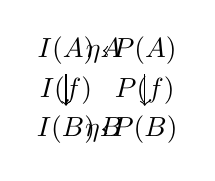
\begin{tikzpicture}
        \node (f a)                {$\funcO{I}(A)$};
        \node (f b) [below of=f a] {$\funcO{I}(B)$};
        \node (g a) [right of=f a] {$\funcO{P}(A)$};
        \node (g b) [below of=g a] {$\funcO{P}(B)$};

        \draw [->] (f a) to node [swap] {$\funcM{I}(f)$}   (f b);
        \draw [->] (g a) to node        {$\funcM{P}(f)$}   (g b);

        \draw [->] (f a) to node        {$\natO{\eta}{A}$} (g a);
        \draw [->] (f b) to node [swap] {$\natO{\eta}{B}$} (g b);
      \end{tikzpicture}
    \end{center}
    \caption{Naturality of the $\eta$ natural transformation.}
    \label{fig:natural-identity-power-set}
  \end{figure}

\end{example}

\section{Natural Transformations in Haskell}
\label{sec:naturals-haskell}

Polymorphic functions in functional programming correspond to natural
transformations. The kind of polymorphism we refer to is parametric
polymorphism. A parametrically polymorphic or generic function is a
function whose ``parameters can have more than one type.'' Such a
function ``works uniformly on a range of types,'' which is ``achieved
by type parameters'' \parencite[476]{cardelli-wegner-1985}.

In Haskell, polymorphic functions can be thought of as functions
between functors in order to relate them to natural transformations.
Given two functors with type constructors \texthaskell{f} and
\texthaskell{g}, a natural transformation \texthaskell{tau} is a
polymorphic function \texthaskell{tau :: f a -> g a} or, using the
\texthaskell{ExplicitForAll} language option, a family of functions
indexed by Haskell types:
\begin{codehaskell}
tau :: forall a. f a -> g a
\end{codehaskell}
More precisely, each \texthaskell{tau} function is a component of a
natural transformation. The naturality of \texthaskell{tau} is the
commutativity of the diagram in Figure \ref{fig:naturality-haskell},
that is, for all functions \texthaskell{f :: a -> b}:
\begin{codehaskell}
tau . fmap f = fmap f . tau
\end{codehaskell}
An intuitive idea behind naturality is that ``terms evaluated in
related environments yield related values''
\parencite[347]{wadler-1989}.

\begin{figure}[htb]
  \begin{center}
    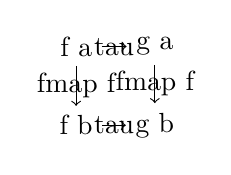
\begin{tikzpicture}
      \node (f a)                {\texthaskell{f a}};
      \node (f b) [below of=f a] {\texthaskell{f b}};
      \node (g a) [right of=f a] {\texthaskell{g a}};
      \node (g b) [below of=g a] {\texthaskell{g b}};

      \draw [->] (f a) to node [swap] {\texthaskell{fmap f}} (f b);
      \draw [->] (g a) to node        {\texthaskell{fmap f}} (g b);

      \draw [->] (f a) to node        {\texthaskell{tau}} (g a);
      \draw [->] (f b) to node [swap] {\texthaskell{tau}} (g b);
    \end{tikzpicture}
  \end{center}
  \caption{Naturality in Haskell.}
  \label{fig:naturality-haskell}
\end{figure}

Naturality in Haskell is the ``theorem for free'' of
\parencite{wadler-1989}, which is also known as parametricity due to
its relation with parametric polymorphism. Given the type of a
polymorphic function, it is possible to conclude that it satisfies its
naturality. However, it is important to note that even though
parametricity guarantees that a polymorphic function satisfies its
naturality, it does not provide a proof of it. Parametricity does not
require the definition of a polymorphic function (only its type), but
proving naturality does.

As examples, we consider the identity natural transformation, the
\texthaskell{head} and \texthaskell{last} functions, which show that
proofs of naturality differ according to the definition, and the
\texthaskell{concat} function, which is one of the examples of
theorems from types in \parencite[349]{wadler-1989}.

\begin{example}
  \label{ex:natural-identity-haskell}

  The identity function of Haskell is a natural transformation.
  Naturality is the identity axiom. See Example
  \ref{ex:natural-identity}, which establishes that the identity
  morphisms are the components of a natural transformation regardless
  of which category it belongs to.

\end{example}

\begin{example}
  \label{ex:natural-head-haskell}

  We have already talked about the \texthaskell{head} function, which
  is a natural transformation from the \texthaskell{[]} (list) functor
  into the \texthaskell{Maybe} functor. Naturality is the
  commutativity of the diagram in Figure
  \ref{fig:naturality-head-haskell}. Here is its proof.

  \vspace{1em}
  \case{\texthaskell{[]}}
  \begin{steps}
    \steph{(head . fmap f) []}
      \eqbydefh{(.)}
    \steph{head (fmap f [])}
      \eqbydefh{fmap}
    \steph{head []}
      \eqbydefh{head}
    \steph{Nothing}
      \eqbydefh{fmap}
    \steph{fmap f Nothing}
      \eqbydefh{head}
    \steph{fmap f (head [])}
      \eqbydefh{(.)}
    \steph{(fmap f . head) []}
  \end{steps}
  \case{\texthaskell{(x:xs)}}
  \begin{steps}
    \steph{(head . fmap f) (x:xs)}
      \eqbydefh{(.)}
    \steph{head (fmap f (x:xs))}
      \eqbydefh{fmap}
    \steph{head (f x : fmap f xs)}
      \eqbydefh{head}
    \steph{Just (f x)}
      \eqbydefh{fmap}
    \steph{fmap f (Just x)}
      \eqbydefh{head}
    \steph{fmap f (head (x:xs))}
      \eqbydefh{(.)}
    \steph{(fmap f . head) (x:xs)}
  \end{steps}

\end{example}

\begin{example}
  \label{ex:natural-last-haskell}

  Another natural transformation from the \texthaskell{[]} (list)
  functor into the \texthaskell{Maybe} functor is the
  \texthaskell{last} function, which extracts the last element of a
  list\footnote{Note that this is not the standard Haskell
    \texthaskell{last} function.}:
  \begin{codehaskell}
last :: [a] -> Maybe a
last []     = Nothing
last (x:[]) = Just x
last (_:xs) = last xs
  \end{codehaskell}
  Its naturality is the commutativity of the diagram in Figure
  \ref{fig:naturality-last-haskell}, that is, for all functions
  \texthaskell{f :: a -> b}:
  \begin{codehaskell}
last . fmap f = fmap f . last
  \end{codehaskell}
  Intuitively, this means that mapping a function over a list and then
  extracting the last element of the list is equivalent to extracting
  the last element of the list and then applying the function. In this
  case, proving naturality requires induction, as follows.

  \begin{figure}[htb]
    \begin{center}
      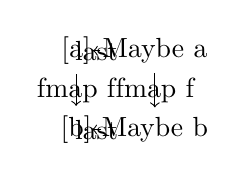
\begin{tikzpicture}
        \node (f a)                {\texthaskell{[a]}};
        \node (f b) [below of=f a] {\texthaskell{[b]}};
        \node (g a) [right of=f a] {\texthaskell{Maybe a}};
        \node (g b) [below of=g a] {\texthaskell{Maybe b}};

        \draw [->] (f a) to node [swap] {\texthaskell{fmap f}} (f b);
        \draw [->] (g a) to node        {\texthaskell{fmap f}} (g b);

        \draw [->] (f a) to node        {\texthaskell{last}}   (g a);
        \draw [->] (f b) to node [swap] {\texthaskell{last}}   (g b);
      \end{tikzpicture}
    \end{center}
    \caption{Naturality of the \texthaskell{last} function.}
    \label{fig:naturality-last-haskell}
  \end{figure}

  \vspace{1em}
  \case{\texthaskell{[]}}
  \begin{steps}
    \steph{(last . fmap f) []}
      \eqbydefh{(.)}
    \steph{last (fmap f [])}
      \eqbydefh{fmap}
    \steph{last []}
      \eqbydefh{last}
    \steph{Nothing}
      \eqbydefh{fmap}
    \steph{fmap f Nothing}
      \eqbydefh{last}
    \steph{fmap f (last [])}
      \eqbydefh{(.)}
    \steph{(fmap f . last) []}
  \end{steps}
  \case{\texthaskell{[x]}}
  \begin{steps}
    \steph{(last . fmap f) (x:[])}
      \eqbydefh{(.)}
    \steph{last (fmap f (x:[]))}
      \eqbydefh{fmap}
    \steph{last (f x : fmap f [])}
      \eqbydefh{fmap}
    \steph{last (f x : [])}
      \eqbydefh{last}
    \steph{Just (f x)}
      \eqbydefh{fmap}
    \steph{fmap f (Just x)}
      \eqbydefh{last}
    \steph{fmap f (last (x:[]))}
      \eqbydefh{(.)}
    \steph{(fmap f . last) (x:[])}
  \end{steps}
  \case{\texthaskell{(x:y:ys)}}
  \begin{steps}
    \steph{(last . fmap f) (x:y:ys)}
      \eqbydefh{(.)}
    \steph{last (fmap f (x:y:ys))}
      \eqbydefh{fmap}
    \steph{last (f x : fmap f (y:ys))}
      \eqbydefh{last}
    \steph{last (fmap f (y:ys))}
      \eqbydefh{(.)}
    \steph{(last . fmap f) (y:ys)}
      \eqbyihh{}
    \steph{(fmap f . last) (y:ys)}
      \eqbydefh{(.)}
    \steph{fmap f (last (y:ys))}
      \eqbydefh{last}
    \steph{fmap f (last (x:y:ys))}
      \eqbydefh{(.)}
    \steph{(fmap f . last) (x:y:ys)}
  \end{steps}

\end{example}

\begin{example}
  \label{ex:natural-concat-haskell}

  We can think of the \texthaskell{concat} function, which
  concatenates a list of lists, as a natural transformation from the
  \texthaskell{[] . []} functor and into the \texthaskell{[]} functor. The type
  signature of this function is:
  \begin{codehaskell}
concat :: [[a]] -> [a]
  \end{codehaskell}
  In this case, naturality is given by, for all functions
  \texthaskell{f :: a -> b}:
  \begin{codehaskell}
fmap f . concat = concat . fmap (fmap f)
  \end{codehaskell}
  That is, the diagram in Figure \ref{fig:naturality-concat-haskell}
  is commutative, which holds by parametricity.

  \begin{figure}[htb]
    \begin{center}
      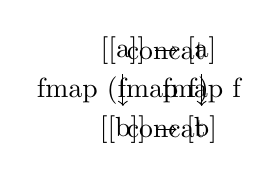
\begin{tikzpicture}
        \node (f a)                {\texthaskell{[[a]]}};
        \node (f b) [below of=f a] {\texthaskell{[[b]]}};
        \node (g a) [right of=f a] {\texthaskell{[a]}};
        \node (g b) [below of=g a] {\texthaskell{[b]}};

        \draw [->] (f a) to node [swap] {\texthaskell{fmap (fmap f)}} (f b);
        \draw [->] (g a) to node        {\texthaskell{fmap f}}        (g b);

        \draw [->] (f a) to node        {\texthaskell{concat}}   (g a);
        \draw [->] (f b) to node [swap] {\texthaskell{concat}}   (g b);
      \end{tikzpicture}
    \end{center}
    \caption{Naturality of the \texthaskell{concat} function.}
    \label{fig:naturality-concat-haskell}
  \end{figure}

\end{example}

\section{References}
\label{sec:naturals-references}

The definition of a natural transformation is based on
\parencites[16]{maclane-1998}[435--436]{poigne-1992}, the \nat{\eta}
natural transformation is taken from \parencite[11]{marquis-2013}, and
the statement that polymorphic functions in functional programming
correspond to natural transformations is based on, for instance,
\parencites[34]{bird-demoor-1997}[78]{elkins-2009}[435,
  436]{poigne-1992}[48,
  49]{rydeheard-1986}[113]{rydeheard-burstall-1988}[350]{wadler-1989}.

\clearemptydoublepage
